% %%%%%%%%%%%%%%%%%%%%%%%%%%%%%%%%%%%%%%%%%%%%%%%%%%%%%%%%%%%%%%%%%%%%%%%%%%%%
\chapter{Dialogue modeling}%
\label{chap:modeling}
% %%%%%%%%%%%%%%%%%%%%%%%%%%%%%%%%%%%%%%%%%%%%%%%%%%%%%%%%%%%%%%%%%%%%%%%%%%%%
Modeling a dialogue is a fairly complicated task which needs to handle communication in natural language as well as  discrete decision process.
Various architectures were proposed over the years, most of which rely on explicit data annotation on multiple levels to guide the model training process.
One of the biggest challenges is to model task-oriented dialogue that requires interaction with external interfaces s.a. databases or API services.
This aspect puts a hard constraint on the dialogue system architecture -- it requires some kind of explicit representation that allows to communicate with external systems.
It's challenging to achieve this in fully unsupervised setting, however, we explore some of the approaches in this chapter.
First, we discuss the challenges of unsupervised task-oriented dialogue modeling in more detail in Section \ref{04:to-unsup}.
Next, we propose our architecture that uses latent representations and explore its abilities and perfromance in Section \ref{04:latent-models}.
Finally, we discuss the usage of Large Language Models as dialogue models and try to answer a question if the usage of these models is able to close the gap between unsupervised and supervised systems.

\section{Task-oriented dialogue modeling with less supervision}
\label{04:to-unsup}
In this section we discuss some of the features we expect from a task-oriented dialogue and how challenging it is to implement them in an unsupervised setting.

\subsection{NLU}
\subsection{External interfaces}
Task-oriented dialogue systems must provide accurate and complete information based on user requests, which requires external database interaction.
%In order to do that, the system needs some form of external database interaction.
%
A turn-level annotation of database queries would represent a similar amount of annotation as is used in supervised training, and thus would not lead to our desired setting, where the model is trained without labeled data.
To support database access while avoiding costly turn-level annotation, we follow \citet{bordes2016learning} and 
insert sparse database queries and results directly into the training data, forming special dialogue turns.
Specifically, we identify turns that require database results, e.g.\ to inform about entity attributes or a number of matching entities, and insert a query-result pair in front of those turns (see Table~\ref{table:example}). We argue that this is the minimal level of supervision required to successfully operate a task-oriented system with database access; it is significantly lower than the full dialogue-state supervision used by most systems.
In addition, it is easily available in the wild (e.g., call center transaction logs).
In practice, we observe that database queries are only inserted for 24\% turns\footnote{This is the average over all datasets in our experiments. Per-dataset query counts are 36\%, 23\% and 11\% for CamRest676, MultiWOZ and SMD respectively.} on average.
Note that this approach still covers the task of an explicit state tracker since the necessary entity values are provided when needed.
To maintain consistency, database query results can be stored and used in follow-up questions.
\begin{table*}[t]
    \centering\scriptsize
    \begin{tabular}{crp{0.6\linewidth}}
        \toprule
         \multirow{4}{*}{\bf Turn 1}&\bf user:& \texttt{Is there a \textbf{moderately priced} restaurant serving \textbf{italian} food anywhere in town?} \\
         &\bf system gold: & \texttt{query italian moderate} \\
         &\bf action: & \texttt{QUERY()} \\
         &\bf system hyp: & \texttt{query \textbf{\textcolor{darkgreen}{italian moderate}}}  \\
         \midrule
        \multirow{4}{*}{\bf Turn 2}&\bf user/database:& \texttt{pizza express, Regent Street City Centre, 01223 324033, C.B 2, 1 D.B, centre}  \\
         &\bf system gold:& \texttt{Pizza express serves italian food and is located in the town centre and is in the moderate price range .} \\        
        &\bf action: & \texttt{OFFER()} \\
        &\bf system hyp:& \texttt{\textbf{\textcolor{red}{Pizza hut Cherry Hinton}} is a italian restaurant in the \textbf{\textcolor{darkgreen}{centre}} part of town} \\
         \midrule
        \multirow{4}{*}{\bf Turn 3}&\bf user:& \texttt{what is the \textbf{address} and \textbf{phone number} ?} \\
        &\bf system gold:& \texttt{their address is  Regent Street City Centre. their phone number is 01223 324033. can i help with anything else ?} \\
         &\bf action: & \texttt{GIVE\_DETAILS()} \\
        & \bf system hyp:& \texttt{the phone number is \textbf{\textcolor{darkgreen}{01223 324033}}. There anything else i can help you with ?} \\
        \bottomrule
    \end{tabular}
    \vspace{-2mm}
    \caption{An example dialogue drawn from the CamRest676 validation set, illustrating the use of database information. We show the user input (or inserted database results), the gold-standard system response, system action annotation based on manual rules and a prediction of our system (Ours-attn configuration using the database, cf.~Table~\ref{04:automatic_metrics_1}). In the first turn, a database query is constructed, the second turn illustrates how the result is retrieved and fed as input. Values inferred correctly by our system are depicted in green, wrong inference is in red.}
    \label{04:tab:example}
\end{table*}
\subsection{Policy decisions}
\section{Latent Dialogue Models}

\subsection{Task-Oriented dialogue with VRNNs}
\begin{figure}[t]
    \centering
    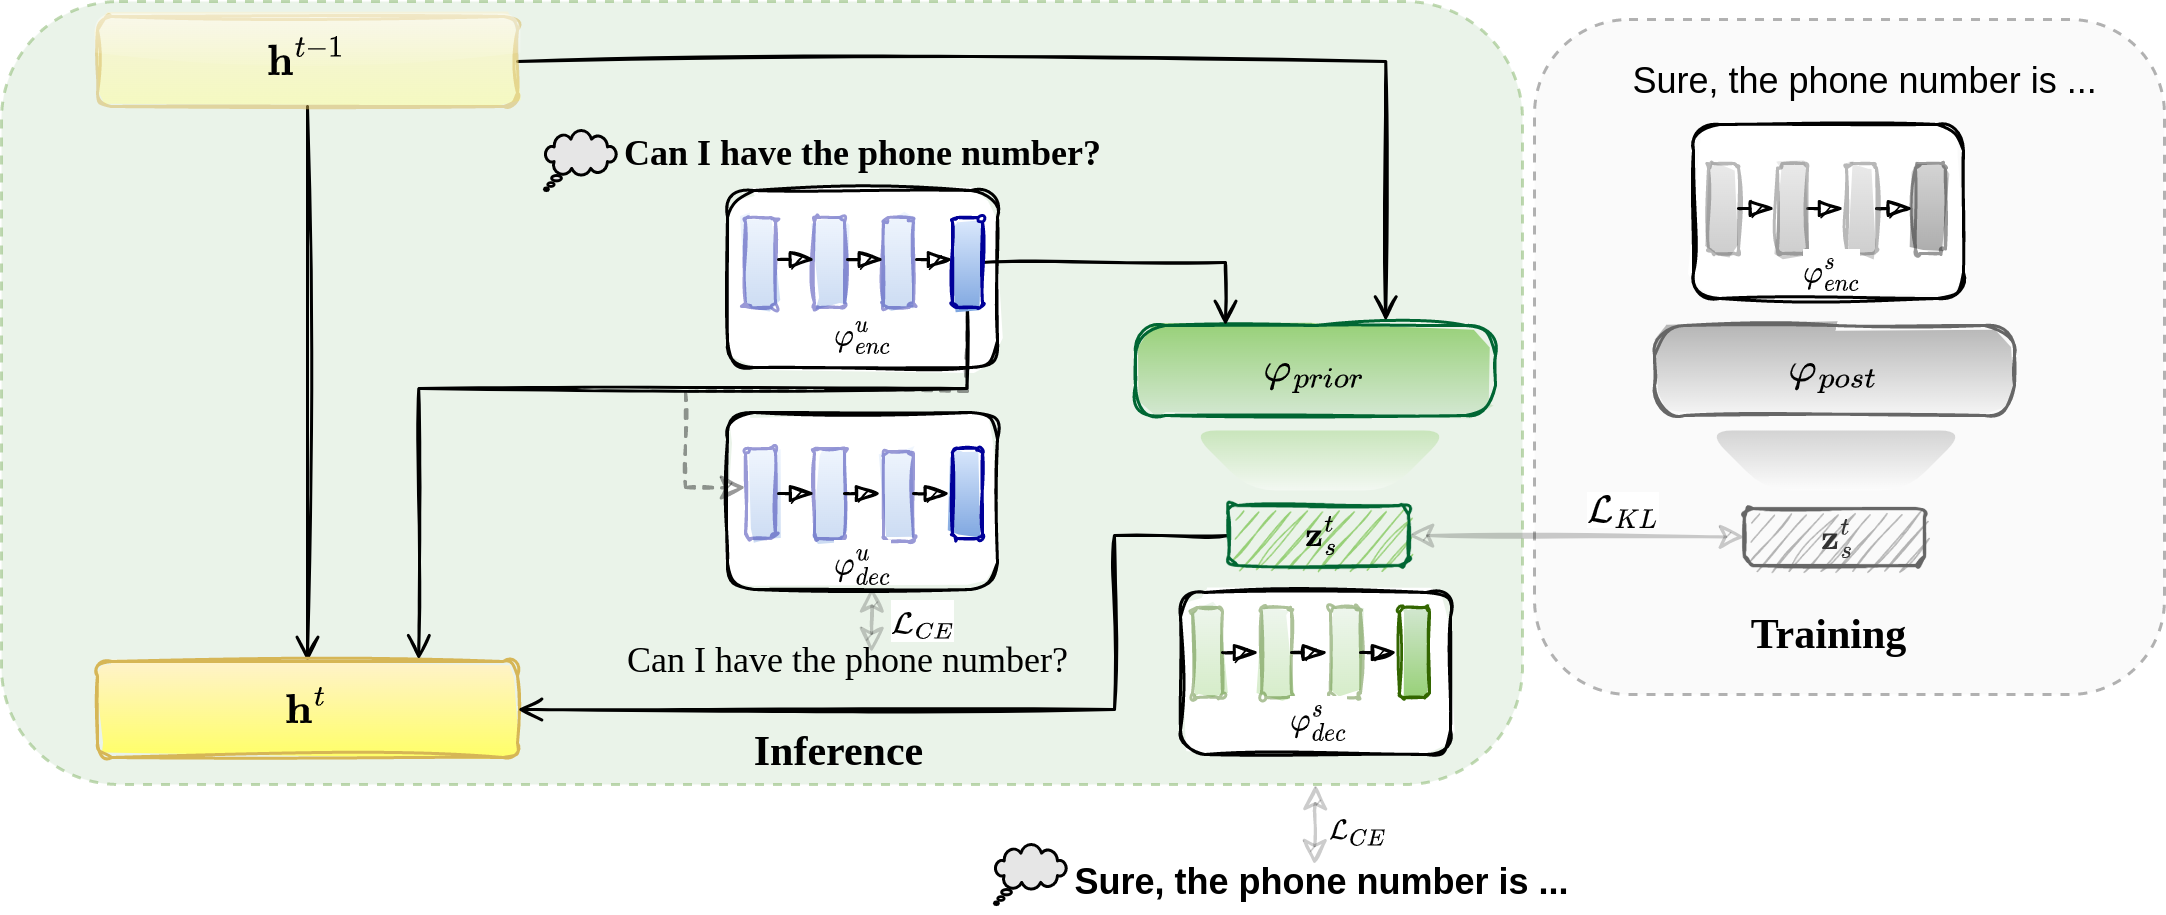
\includegraphics[width=0.9\textwidth]{images/vrnn-paper.png}
    \caption{Visualization of our model architecture (one dialogue turn). Yellow boxes represent the turn-level VRNN's hidden state $h^t$. The user utterance is represented as the last hidden state of the encoder network $\varphi_{enc}^u$, which is trained as an autoencoder along with the decoder $\varphi_{dec}^u$. The system utterance, encoded by the network $\varphi_{enc}^s$, is an input to the posterior network $\varphi_{post}$ that helps to train the prior network $\varphi_{prior}$ to construct meaningful latent variables $\mathbf{z}_s$, which initialize the system utterance decoder $\varphi_{dec}^s$. Training uses the whole architecture, including the posterior network $\varphi_{post}$, while only uses the part shaded in green is used for inference.} $\mathcal{L}_{CE}$ stands for cross-entropy loss, $\mathcal{L}_{KL}$ for KL-divergence loss.
    \label{fig:vrnn_method}
\end{figure}

We use the VRNN model introduced in Chapter \ref{background:vrnn} and extend it to fit the task-oriented setup.
Our model's architecture is depicted in Figure \ref{fig:vrnn_method}.
We employ a turn-level RNN that summarizes the context to its hidden state.
In each dialogue turn, we model user and system utterances with separate autoencoders to account for different user and system behavior.
The user utterance is modeled with a standard autoencoder; the last encoder hidden state $\varphi^u_{enc}(\mathbf{x}^t_u)$ provides the encoded representation.
For the system part, we use a VAE with discrete latent variables $\textbf{z}_s$ conditioned on the context RNN's hidden state $\mathbf{h}^{t-1}$ and the user utterance encoding $\varphi^u_{enc}(\mathbf{x}^t_u)$.
Our model can thus be seen as a VRNN extended by an additional encoder-decoder module.
The context RNN hidden state update looks as follows:
\begin{equation}
    \begin{gathered}
        \mathbf{h}^{t+1} = \text{RNN}([\varphi^u_{enc}(\mathbf{x}_u^t),\varphi_{z}(\mathbf{z}^t_s)], \mathbf{h}^t)
    \end{gathered}
\end{equation}
For word-level encoding and decoding modules ($\varphi_{enc}^u,\varphi_{enc}^s,\varphi_{dec}^u,\varphi_{dec}^s$), we use an RNN with LSTM cells.
We further experiment with attention \cite{bahdanau2014neural} over user encoder hidden states in the system decoder.
We train the model by minimizing a sum of the cross-entropy reconstruction loss on user utterances and the variational lower bound loss (Equation~\ref{eq:vae}) on system responses.

When running in inference mode, only the prior distribution $p(\mathbf{z}_s)$ is considered, which does not require the system utterance on the input.
Therefore, the model is able to generate the system response when provided with a user utterance on the input.

\paragraph{Latent Variables}
\label{sec:method_latent}
We use a set of $n$ \mbox{$K$-way} $(K=20;n=1,3,5)$ categorical variables to achieve good interpretability, following \citet{zhao2018unsupervised}.
This means that each variable is represented as a one-hot vector of length $K$, and we use $n$ such vectors.
%To achieve good interpretability, we need the distribution to yield discrete values. 
We use the Gumbel-Softmax distribution and the reparameterization trick \cite{jang2017categorical}.
During inference, we apply argmax directly to the predicted distribution, instead of sampling from it.

\subsection{Hierarchical models for task-oriented dialogue}

\section{Experiments and Results}

\begin{table}[t]
    \centering\small
    \begin{tabular}{l|c|cc}
      \toprule
      config & \textbf{CamRest676} & \multicolumn{2}{c}{\textbf{MultiWOZ 2.1.}} \\
       & gold & domain & action \\
      \midrule
      random  & 0.167 & 0.143 & 0.093 \\
      majority &  0.417 & 0.327 & 0.316 \\\hdashline[0.5pt/2pt]
      HRED & 0.645 & 0.445 & 0.437 \\
      VHRED & 0.521 & 0.357 & 0.323 \\
      GPT-2 & 0.650 & 0.601 & 0.552 \\
      %ours-3z & 0.648 & 0.599 & 0.543 \\
      Ours-attn & 0.616 & 0.683 & 0.664 \\
%     ours-5z (LR) & 0.721 &  & \\
      Ours-noattn & \textbf{0.753} &  \textbf{0.704} & \textbf{0.691} \\\hdashline[0.5pt/2pt]
      Ours-manual & 0.587 & -- & -- \\
      %10z (DT) & \textbf{0.759} & \textbf{0.641} & \textbf{0.404} \\
      %10z-attn (DT) & 0.597 & 0.460 & 0.296 \\

      \bottomrule
  \end{tabular}
  \caption{Accuracy of the domain and action decision-tree classifiers based on latent variables. 
  %We use Logistic Regression (LR) and Decision Tree (DT) classifiers for continuous and discrete inputs respectively.
  For details about the manual annotation process, see Section~\ref{sec:manual}.}
  \label{tab:latent_classification}
\end{table}


In this section, we focus on the quality of responses generated by our model as well as on model performance with respect to dialogue task success.
We focus on theoretical modeling and feasibility at this stage, which we believe is sufficiently demonstrated by corpus-based evaluation complemented by manual checks. Detailed interpretation of the learned representations follows in Section~\ref{sec:latents}.

\subsection{Data}
\label{sec:data}

We evaluate the model performance on three datasets: CamRest676 \cite{wen2016network}, MultiWOZ 2.1 \cite{budzianowski2018multiwoz,eric2019multiwoz} and Stanford Multidomain Dialogues \cite[SMD;][]{eric-etal-2017-key}\footnote{We use standard splits for MultiWOZ 2.1 and SMD. We split CamRest676 in the 8:1:1 ratio, following previous work.}
Detailed descriptions are given in Section \ref{02:sec:input-data-desc}.

\paragraph{Database queries} To include database information in the dialogues, we first identify all turns in the original datasets where database information is required, using handcrafted rules.\footnote{These rules are very simple and require minimal effort: whenever database results are provided in the data (based on simple pattern matches over system actions), we prepend a database query based on ground-truth state. The assumption is that in a real-world scenario, these queries would naturally be available -- database queries induced by human operators can be logged along with client-operator conversations.}
We then build database query turns based on the respective state annotation (see example in Table~\ref{tab:example}).
Note that database query parameters are the only annotation used to train our models apart from utterance texts; no other dialogue state annotation from the original datasets is used.
%We acknowledge that this approach provides a certain amount of weak supervision to the system; however, it reflects the intended use case of our system, i.e. automating a call center based on recordings of previous human-human dialogues.
\subsection{Experimental Setup}
\label{sec:expe_setup}
%We release our code along with this paper.\footnote{Link removed for anonymity.}
We evaluate two versions of our model: one that uses the attention mechanism (\emph{attn}) and one without it (\emph{noattn}). The number and size of the variables are set based on a few cursory checks on the training data. Our models use 10 latent variables by default; we discuss the influence of the number of latent variables in Table \ref{04:z_counts}.
Since our approach is the first to be evaluated in a task-oriented setting with this minimal level of supervision, comparing to prior works is difficult. Setups with full dialog state supervision are not comparable and dialog-state metrics are not applicable without the turn-level supervision. Therefore, we compare our models to standard architectures, such as vanilla LSTM or Transformer encoder-decoder, predicting in a sequence-to-sequence fashion using the same amount of supervision as our approach. We also compare to the HRED/VHRED models, which are perhaps the closest prior work to our approach. To put the results into perspective, we also include scores for fully supervised state of the art on our datasets.
However, note that these scores are not directly comparable.
\footnote{The training is sensitive to some parameters, such-as the \nobreak{Gumbel-softmax} temperature, but otherwise the model trains easily using conventional optimization methods.}

\begin{table}[ht]
    \centering\small
    \begin{tabular}{l|c|rrrr|rrrr}
      \toprule
      model &  & \multicolumn{4}{c|}{\textbf{CamRest676}}  & \multicolumn{4}{c}{\textbf{MultiWOZ~2.1}} \\
      & db & BLEU & Ppl & MI & EMR &  BLEU & Ppl & MI & EMR \\
    LSTM & \textcolor{red}{\xmark} & 3.90 & 5.34 & -- & -- &  0.92 & 8.23 &
    -- & --\\
    Transformer & \textcolor{red}{\xmark} & 4.98 & 7.72 & -- & -- & 0.95 & 6.95 & -- & -- \\
    GPT-2 & \textcolor{red}{\xmark} & 15.40  & 1.18 & -- & -- & 9.40 & 2.77 & -- & -- \\
    GPT-2 & \textcolor{green}{\cmark} & 13.89 & 1.80 & -- & -- & 9.56 & 2.43 & -- & -- \\
    HRED & \textcolor{red}{\xmark} & \pz2.70 & 13.92 & -- & 0.02 & \pz2.98 & 29.61 &
    -- & 0.01\\
    VHRED & \textcolor{red}{\xmark} & \pz4.34 & 11.76 & 0.21 & 0.02 & \pz4.65 & 32.74 & 0.15 & 0.01 \\
    VHRED & \textcolor{green}{\cmark} & \pz8.50 & 10.23 & 0.17 & 0.36 & 3.82 & 16.61 & 0.07 & 0.04 \\
    \hdashline[0.5pt/2pt]
    Ours-noattn & \textcolor{red}{\xmark} & 12.98 & \pz4.64 & 0.29 & 0.01 & \pz7.18 & \pz9.16 & \bf0.42 & 0.02\\
    Ours-noattn & \textcolor{green}{\cmark} & 15.10 & \pz4.45 & \bf0.34 & 0.24 &  11.3 & \pz5.17 & 0.27 & 0.05\\
    Ours-attn & \textcolor{red}{\xmark} & \bf17.37 &\pz 5.07 & 0.16 &  0.09 & \bf12.28 & 10.19 & 0.06 & 0.04\\
    Ours-attn & \textcolor{green}{\cmark} & 17.10 & \pz\bf4.23 & 0.22 & \bf0.81 & 11.86 & \bf\pz6.03 & 0.05 & \bf0.08\\
    \hdashline[0.5pt/2pt]
    \emph{supervised $^{*}$} & \textcolor{green}{\cmark} & 25.50  & -- & -- & -- & 19.40 & 2.50 & -- & -- \\
    \bottomrule
  \end{tabular}
  \caption{Model performance in terms of Entity Match Rate, BLEU for generated responses, Perplexity (Ppl), and Mutual Information (MI) between the generated response and the latent variables $\mathbf{z}_s$. 
  %We do not evaluate the database-enriched models on SMD as SMD's database structure does not map easily to our annotation style. 
  We measure MI only for the models that use latent variables explicitly. The \emph{db} column indicates systems that use database information. $^{*}$Note that the supervised state-of-the-art scores are not directly comparable, as the systems use full turn-level supervision. Systems listed: CamRest676 \cite{peng2021soloist};  MultiWOZ \cite{lin2020mintl}.}
  \label{04:automatic_metrics_1}
\end{table}
\begin{table}[ht]
    \centering\small
    \begin{tabular}{l|c|rrr}
      \toprule
      model &  & \multicolumn{3}{c}{SMD} \\
      & db & BLEU & Ppl & MI  \\
    LSTM & \textcolor{red}{\xmark} & 1.62 & 7.84 & -- \\
    Transformer & \textcolor{red}{\xmark}  & 1.53 & 6.33 & -- \\
    GPT-2 & \textcolor{red}{\xmark} & 9.26 & 2.46 & -- \\
    GPT-2 & \textcolor{green}{\cmark} & 4.54 & 2.02 & -- \\
    HRED & \textcolor{red}{\xmark} & \pz1.25 & 12.50 & -- \\
    VHRED & \textcolor{red}{\xmark} & \pz3.75 & 11.94 & 0.20 \\
    VHRED & \textcolor{green}{\cmark} & 3.94 & 11.86 & 0.19 \\
    \hdashline[0.5pt/2pt]
    Ours-noattn & \textcolor{red}{\xmark} & \pz7.35 & \pz6.18 & \bf0.53 \\
    Ours-noattn & \textcolor{green}{\cmark} & \pz9.24 & \pz\bf6.01 & 0.47 \\
    Ours-attn & \textcolor{red}{\xmark} & 12.30 & \pz6.36 & 0.04 \\
    Ours-attn & \textcolor{green}{\cmark} & \bf12.40 & 6.11 & 0.11 \\
    \hdashline[0.5pt/2pt]
    \emph{supervised$^{*}$} & \textcolor{green}{\cmark}& 14.40 & -- & --  \\
    \bottomrule
  \end{tabular}
  \caption{Model performance in terms of BLEU for generated responses, Perplexity (Ppl), and Mutual Information (MI) between the generated response and the latent variables $\mathbf{z}_s$. 
  We do not evaluate the database-enriched models on SMD as SMD's database structure does not map easily to our annotation style. 
  We measure MI only for the models that use latent variables explicitly. The \emph{db} column indicates systems that use database information. $^{*}$Note that the supervised state-of-the-art scores are not directly comparable, as the systems use full turn-level supervision. Systems listed: SMD \cite{qin2020dynamic}; }
  \label{04:automatic_metrics_2}
\end{table}
\subsection{Response quality}
To evaluate the quality of individual responses, we compute BLEU score \cite{papineni2002} and perplexity on the test set (see Tables~\ref{04:automatic_metrics_1},\ref{04:automatic_metrics_2 }).

Our architecture performs substantially better than (V)HRED, which commonly fails to pick up the necessary knowledge, especially on larger datasets.
The attention-based versions perform better on BLEU, but lose slightly on perplexity.
Comparing HRED and VHRED shows that using the variational approach generally improves overall performance.
While the GPT-2 PLM outperforms our approach on perplexity, it is worse on BLEU score, despite its huge capacity.

We compare to other relevant related works:
\begin{enumerate}
\item \citet{shi2019unsupervised} do not use their model for response generation, but they report a negative log likelihood of approximately $5.5 \cdot 10^{4}$ when reconstructing the CamRest676 test set. Our \emph{Ours-noattn} model obtained $0.87 \cdot 10^{4}$, which suggests a better fit of the data.\footnote{This comparison is only approximate since the exact data split is not described by \citet{shi2019unsupervised} -- we are only able to use a test set of the same size, not the exact same instances.}
\item \citet{wen2017latent} measure response generation BLEU score on fully delexicalized CamRest676 data. Their best reported result is 24.60, while our model gets 27.23 (30.10 with attention).
\end{enumerate}

Based on manual checks,
our models are able to generate relevant responses in most cases.
As expected, only the models including database turns are able to predict correct entities (cf.~Section~\ref{sec:emr}).
A relatively common error is informing about wrong slots, e.g.\ the model provides a phone number instead of an address or, even more frequently, provides wrong slot values (cf.~Table~\ref{04:tab:example}).
%An example of such a situation is highlighted in Table~\ref{tab:example}.

\begin{table}[t]
    \centering\small
    \begin{tabular}{lcc}
      \toprule
      model &  success & query acc.\hspace{-2mm} \\
      \midrule
      \multicolumn{3}{c}{\textbf{CamRest676}} \\
      \midrule
      VHRED & 0.21 & 0.91 \\
      Ours-noattn & 0.28 & 0.84 \\\hdashline[0.5pt/2pt]
      supervised SotA \cite{peng2021soloist}\hspace{-2mm} & 0.73 & N/A \\
      \midrule
      \multicolumn{3}{c}{\textbf{MultiWOZ}} \\
      \midrule
      Ours-noattn & 0.10 & 0.98 \\\hdashline[0.5pt/2pt]
      supervised SotA \cite{peng2021soloist}\hspace{-2mm} & 0.85 & N/A \\
      \bottomrule
  \end{tabular}
  \caption{Dialogue success and query accuracy comparison for VHRED, \emph{Ours-noattn} using the database and a state-of-the-art supervised system.}
  \label{tab:success}
\end{table}

\subsection{Task-related performance}
\label{sec:succ}
Without dialogue-state supervision, we cannot measure task-oriented metrics such as \emph{inform} rate or \emph{joint goal accuracy}.
Therefore, we decided to measure dialogue success and entity match rate, which we adjust to the minimally supervised case (details follow). We also measure database query accuracy.

\paragraph{Dialogue success}
%Traditionally, task-oriented dialogue systems are evaluated with  the \emph{dialogue success} metric.
The dialogue success or \emph{success rate} reflects the ratio of dialogues in which the system captures all the mentioned slots correctly and provides all the requested information.
We follow previous works \cite{nekvinda2021shades} and report corpus-based success score, as opposed to using a user simulator.
However, measuring success rate without turn-level labels is not straightforward. % if no slot labels are available.
%This is simpler to set up and does not depend on simulator quality.
%
We approximate tracking slot values turn-by-turn by checking for correct slot values upon database queries only, and we use this information to measure dialogue success.
Note that this is not equivalent to having state tracking labels available at all turns, but we consider it a reasonable approximation given our limited supervision -- database queries are crucial for presenting the correct entities to the user, which in turn decides the dialogue success.
%Since we include database queries in our dataset, we are able to obtain all the information necessary to measure this approximation of success rate.
The generated query attributes directly show the captured slots.
%Because we have no access to the correct state labels in the unsupervised setting, we determine the entity attributes from the database queries and use the attributes to measure the success rate.

Success rate results are shown in Table~\ref{tab:success}.
Our system is not competitive with a fully supervised model, but outperforms the baselines (VHRED, GPT).
Upon inspection,
we see that the system is often able to recognize correct slots, however, it has difficulties capturing the correct values.
%Also, there is a large gap between our results and the fully supervised system.
However, the scores  are promising considering the minimal supervision of our training.

\paragraph{Matching database entities}
\label{sec:emr}
To evaluate the accuracy of the offered entities, we measure the Entity Match Rate (EMR), i.e. the ratio of generated responses with correct entities over all responses that mention some entity.
Table~\ref{tab:automatic_metrics} shows  the results.
We observe that the model performance without the database information is poor.
However, including the database information improves the performance substantially, especially in the case of CamRest676 data.
The MultiWOZ data is much more complex -- it contains more slots and multiple domains that can also be combined in an individual dialogue.
Nevertheless, we can still observe an improvement when we include the database queries.
We also note that using attention improves EMR substantially -- the latent variables alone cannot hold all information about particular values (cf.~Section~\ref{sec:pred_latents}).

\paragraph{Database query accuracy}
Further, we evaluate the accuracy of the database querying.
This metric simply measures if the system queries the database at appropriate turns.
The content of the query is not taken into account in this case, as it is already considered in the success rate. On MultiWOZ, we get a near-perfect accuracy, while our approach loses to VHRED on CamRest676 (see Table~\ref{tab:success}).
We hypothesize that this discrepancy can be caused by different dialogue structures among theses two datasets. The dialogues in CamRest676 usually contain just zero or one query during a dialogue, so our model might generate more queries than necessary.

\section{Latent Variable Interpretation}
\label{sec:latents}
\begin{table}[h]
    \centering\small
    \begin{tabular}{l|ccc}
      \toprule
      & BLEU & Ppl & MI  \\
    \midrule
    Ours-noattn-1z  & 25.2 & 4.25 & 0.46  \\
    Ours-noattn-3z  & 26.8 & 4.24 & 0.26  \\
    Ours-noattn-5z  & 27.23 & 4.20 & 0.38  \\
    Ours-noattn-12z  & 29.83 & 4.12 & 0.35  \\    

    \bottomrule
  \end{tabular}
  %\vspace{-2mm}
  \caption{Evaluation of the model performance with respect to automatic measures of BLEU, Perplexity (Ppl) and Mutual Information (MI) on the CamRest676 data.}
  \label{04:z_counts}
\end{table}
We believe that being able to explain and interpret the model behavior is crucial, especially in a setting without full supervision.
Therefore, we design a set of experiments to evaluate the model behavior and investigate whether the model captures salient dialogue features in the latent variables obtained during training on CamRest676 and MultiWOZ.
While it seems that the latent variables are mainly useful for interpretability or structure induction, they are likely also contributing to the performance as smaller latent spaces yield lower performance as we can see in Table \ref{04:z_counts}.

\subsection{Clustering the actions}
\label{sec:clustering}
First, we want to assess whether similar variables represent similar actions.
We follow \citet{zhao2018unsupervised} and define utterance clusters according to the latent variables that have been assigned to them by the model.
We then use the homogeneity metric \cite{rosenberg-hirschberg-2007-v} to evaluate the clustering quality with respect to the reference classes determined by manually annotated system actions (which are used for evaluation only).
Homogeneity reflects the amount of information provided by the clustering (and by extension, the latent vectors used) and is normalized to the interval [0, 1].
The reason of choosing this metric is that it is independent on the number of labels and their permutations.
%If all clusters only contain instances of a single class, we get the maximum homogeneity.
We provide the results in Table~\ref{tab:homo}.
The clusters formed on the CamRest676 data are more homogeneous than on MultiWOZ, likely because of the greater dataset complexity in the latter case. 
In all cases, our clusters are much more homogeneous than clustering formed by random assignment.
We also compare favorably to stronger baseline that is based on clustering of the sentence representations.
Specifically, in this approach we compute sentence representations using a BERT model tuned for sentence representations \cite{reimers-2019-sentence-bert} and then cluster the obtained sentence embeddings using K-means clustering.

\begin{figure*}[t]
    \centering
    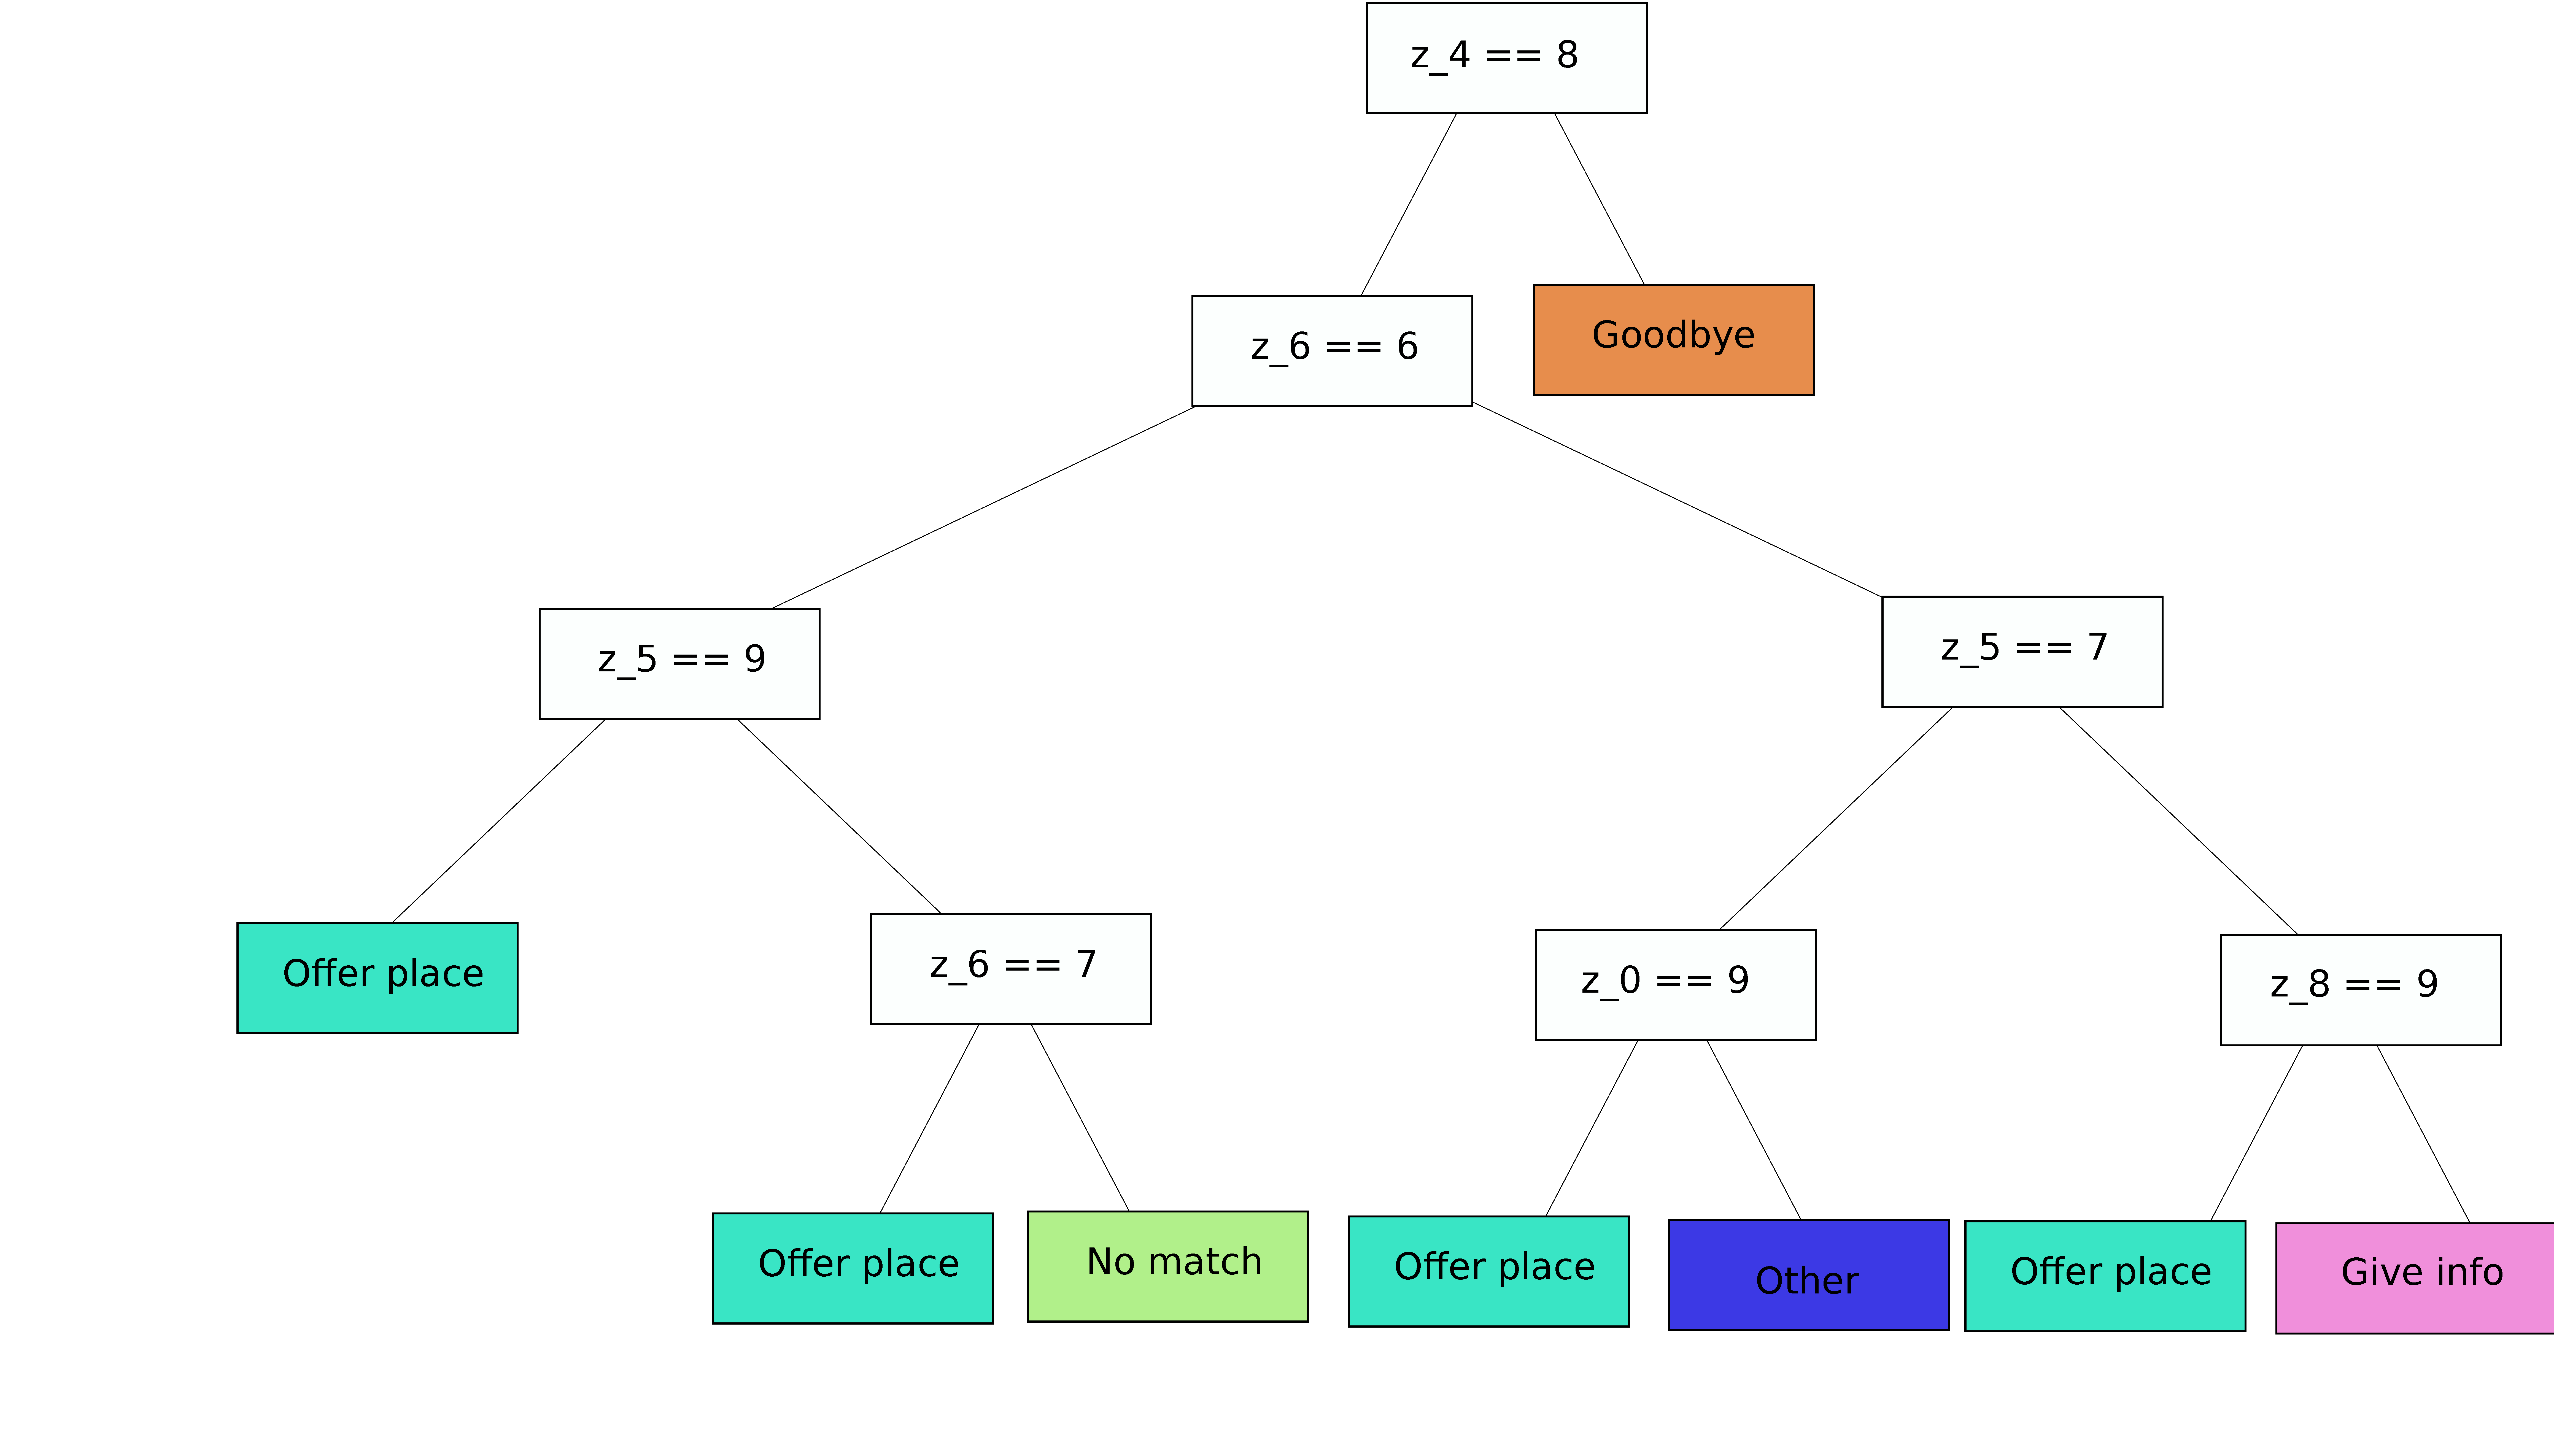
\includegraphics[width=0.70\textwidth]{images/dt2.pdf}
    \vspace{-5mm}
    \caption{A visualization of a decision tree trained on the CamRest676 data to predict a system action from the contents of the latent variables. Each node represents a decision based on one latent variable value and the leaf node colors represent different system actions. When the condition in a given node is fulfilled, the algorithm proceeds into the right subtree, left otherwise. For clarity, we limit the maximum tree depth to 4. The limit lowers the accuracy slightly -- the pictured tree achieves an accuracy of 73\% on the CamRest676 data.}
    \label{fig:dt}
\end{figure*}

\subsection{Predictive power of the variables}
\label{sec:pred_latents}
To evaluate the predictive power of the obtained latent representations, we train a simple classifier that predicts the system action and current domain, using solely the obtained latent representations as input features.
CamRest676 data does not include system action annotation, hence we manually designed a set of rules to determine system actions.
An example of this rule-based action annotation is shown in Table~\ref{04:tab:example}.
For MultiWOZ, we predict both system action and the domain of the utterance.
%We hypothesize that a good representation should capture the information about dialogue system state.

To put our results into perspective, we include several baselines: trivial random and majority class baselines, and classifiers using representations obtained with other methods (HRED, VHRED, GPT).
We use a decision tree (DT) classifier trained with the CART algorithm\footnote{\url{https://scikit-learn.org/stable/modules/tree.html}} and the \emph{gini} split criterion, due to the its good interpretability.
The results are shown in Table~\ref{tab:latent_classification}.
Our classifier beats the random and majority baselines in all cases.
More importantly, it also outperforms classification based on (V)HRED and GPT representations.
This demonstrates that our approach produces high-quality interpretable representations.
We also observe that using attention harms the performance of the action classifier as it makes it possible for the models to bypass the latent variables.
%On CamRest676, the latent variables explain the vast majority of the annotated actions.
%Overall, we can obsereve that any hidden state taken from some trained model can explain some portion of the data.
%However, using our approach seem to perform better in this aspect.
%We also notice the influence of the number of latent variables used on the performance.
%In general, increasing the number of latent variables leads to a substantial performance improvement, which suggests that all the variables contribute with relevant information (see Table~\ref{tab:latent_classification}).

The information about domains and system actions is stored in categorical variables and can be extracted by a simple classification model such as the decision tree which allows us to interpret and explain the behavior of our model.
For illustration, in Figure \ref{fig:dt} we plot a DT with limited depth that achieves 73\% accuracy when predicting the system action on the CamRest676 data.\footnote{The aim is that latent variables hold high-level information, such as intents, actions or domains. This helps interpretability, but is not sufficient for generating appropriate and factually correct responses -- here we need to incorporate correct slot values. This detailed information is captured and carried over via the attention mechanism in \emph{Ours-attn}. Potential alternatives are copy mechanisms \cite{lei2018} or delexicalization on the generated outputs \cite{henderson_robust_2014,peng2021soloist}.}

\subsection{Manual interpretation}
\label{sec:manual}
To explore the interpretability of our representations even further, we manually annotate the latent variables to obtain a simple handcrafted classifier.
Specifically, we draw a set of pairs of utterances and corresponding latent representations from the validation set.
Then we present the representation (discrete) vectors to an expert annotator with a task of assigning an action that each vector represents, based on the sampled utterances.
This way we obtain a mapping from the space of latent vectors to actions.
We then apply this mapping to predict actions on the test set (the \textit{-manual} entry in Table \ref{tab:latent_classification}).
Note that in this approach, we only allow assigning an action to a whole vector, unlike in the case of decision tree classifier that can take individual components into account.
As the results show, this approach works well, despite the above limitation.

\begin{table}[t]
    \centering\small
    \begin{tabular}{l|c|c|c}
      \toprule
      \textbf{Target} & Ours-noattn & sent-repr & random \\
      \midrule
      CamRest676 action & 0.65 & 0.45 & 0.20\\
      MultiWOZ action & 0.34 & 0.33 & 0.02\\
      MultiWOZ domain & 0.39 & 0.30 & 0.01 \\
      \bottomrule
  \end{tabular}
  \caption{Homogeneity for \emph{Ours-noattn} configuration using the database vs.~a clustering of sentence representations and random baseline.}
  \label{tab:homo}
\end{table}

\subsection{Mutual Information}
Finally, we compute mutual information (MI) between the generated text and latent variables as well as among the latent variables themselves (see Table~\ref{04:automatic_metrics_1}).\footnote{
Since we measure MI between categorical variables, we quantize the continuous variables used in the VHRED model.}
We see that using attention has a dramatic effect on the amount of MI between the latent variables and the generated text. % It seems that the since
It appears that since attention bypasses the latent vectors, the decoder does not need to use them to store information.
